\begin{figure}
    \centering
    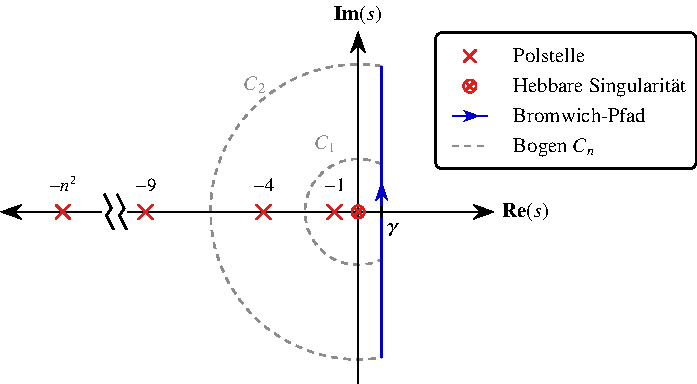
\includegraphics{papers/laplace/images/pol_kette.pdf}
    \caption{Die Singularitäten des Stabes endlicher Länge:
    unendlich viele einfache Pole bei $s_\nu = -\nu^2$ auf der negativen
    reellen Achse.
    Die Abstände wachsen quadratisch, die Wellenlinie deutet die
    Fortsetzung der Kette bis zum $n$-ten Pol und darüber hinaus an.
    Die gestrichelten Bögen $C_n$ verlaufen jeweils zwischen zwei Polen
    und schliessen den Bromwich-Pfad für die Residuenauswertung.}
    \label{laplace:fig:pol_kette}
\end{figure}
